\documentclass[10pt,ignorenonframetext,]{beamer}
\setbeamertemplate{caption}[numbered]
\setbeamertemplate{caption label separator}{: }
\setbeamercolor{caption name}{fg=normal text.fg}
\beamertemplatenavigationsymbolsempty
\usepackage{lmodern}
\usepackage{amssymb,amsmath}
\usepackage{ifxetex,ifluatex}
\usepackage{fixltx2e} % provides \textsubscript
\ifnum 0\ifxetex 1\fi\ifluatex 1\fi=0 % if pdftex
  \usepackage[T1]{fontenc}
  \usepackage[utf8]{inputenc}
\else % if luatex or xelatex
  \ifxetex
    \usepackage{mathspec}
  \else
    \usepackage{fontspec}
  \fi
  \defaultfontfeatures{Ligatures=TeX,Scale=MatchLowercase}
\fi
\usetheme[]{metropolis}
% use upquote if available, for straight quotes in verbatim environments
\IfFileExists{upquote.sty}{\usepackage{upquote}}{}
% use microtype if available
\IfFileExists{microtype.sty}{%
\usepackage{microtype}
\UseMicrotypeSet[protrusion]{basicmath} % disable protrusion for tt fonts
}{}
\newif\ifbibliography
\hypersetup{
            pdftitle={Markov melding, multi-stage sampling, and self-density ratios},
            pdfauthor={Andrew Manderson},
            pdfborder={0 0 0},
            breaklinks=true}
\urlstyle{same}  % don't use monospace font for urls

% Prevent slide breaks in the middle of a paragraph:
\widowpenalties 1 10000
\raggedbottom

\AtBeginPart{
  \let\insertpartnumber\relax
  \let\partname\relax
  \frame{\partpage}
}
\AtBeginSection{
  \ifbibliography
  \else
    \let\insertsectionnumber\relax
    \let\sectionname\relax
    \frame{\sectionpage}
  \fi
}
\AtBeginSubsection{
  \let\insertsubsectionnumber\relax
  \let\subsectionname\relax
  \frame{\subsectionpage}
}

\setlength{\parindent}{0pt}
\setlength{\parskip}{6pt plus 2pt minus 1pt}
\setlength{\emergencystretch}{3em}  % prevent overfull lines
\providecommand{\tightlist}{%
  \setlength{\itemsep}{0pt}\setlength{\parskip}{0pt}}
\setcounter{secnumdepth}{0}
\usepackage{amsmath}
% I always seem to need tikz for something
\usepackage{tikz}
\usetikzlibrary{positioning, shapes, intersections, through, backgrounds, fit, decorations.pathmorphing}

% \usepackage{setspace}
% \onehalfspacing

\usepackage{lineno}
% \linenumbers

% required for landscape pages. beware, they back the build very slow.
\usepackage{pdflscape}

% table
\usepackage{longtable}
\usepackage{booktabs}
\usepackage{caption}

% \usepackage[colorlinks=true, urlcolor=citecolor, linkcolor=citecolor, citecolor=citecolor]{hyperref}

% cross out math
\usepackage[makeroom]{cancel}

\usepackage{color}
\definecolor{myredhighlight}{RGB}{180, 15, 32}
\definecolor{mydarkblue}{RGB}{0, 33, 79}
\definecolor{mymidblue}{RGB}{44, 127, 184}
\newcommand{\semitransp}[2][35]{\color{fg!#1}#2}

% beamer things
\setbeamercolor{frametitle}{bg=black}
\setbeamerfont{footnote}{size=\tiny}

\setcounter{secnumdepth}{3}

% pd stands for: probability distribution and is useful to distringuish
% marignals for probabilities specifically p(p_{1}) and the like.
\newcommand{\pd}{\text{p}}
\newcommand{\q}{\text{q}}
\newcommand{\w}{\text{w}}
\newcommand{\pdr}{\text{r}}
\newcommand{\pdrh}{\hat{\text{r}}}

% melding
\newcommand{\ppoolphi}{\pd_{\text{pool}}(\phi)}

% the q(x)w(x), "weighted target" density 
% for the moment I'm going to call it s(x), as that is the next letter of the 
% alphabet. Can change it later
\newcommand{\s}{\text{s}}
% direct density estimate - replaces lambda.
\newcommand{\ddest}{\text{s}}

% constants - usually sizes of things
\newcommand{\Nx}{N}
\newcommand{\Nnu}{\text{N}_{\text{nu}}}
\newcommand{\Nde}{\text{N}_{\text{de}}}
\newcommand{\Nmc}{\text{N}_{\text{mc}}}
\newcommand{\Nw}{W}
\newcommand{\Nm}{M}

% locales - could switch to x and x'
\newcommand{\xnu}{x_{\text{nu}}}
\newcommand{\xde}{x_{\text{de}}}
\newcommand{\phinu}{\phi_{\text{nu}}}
\newcommand{\phide}{\phi_{\text{de}}}

% sugiyama stuff
\newcommand{\pdnu}{\pd_{\text{nu}}}
\newcommand{\pdde}{\pd_{\text{de}}}


% indices 
\newcommand{\wfindex}{w}
\newcommand{\sampleindex}{n}
\newcommand{\modelindex}{m}

\title{Markov melding, multi-stage sampling, and self-density ratios}
\author{Andrew Manderson}
\date{2019-10-07}

\begin{document}
\frame{\titlepage}

\begin{frame}{Statistical modelling}

\begin{center}
\begin{tikzpicture}[node distance = 2cm, thick, state/.style={circle, draw, minimum width = 1.5cm, align = center}]
  % nodes
  \node [state] (data) {Data: \\ $Y$};
  \node [state][right = 2.0cm of data] (model) {Model: \\ $\pd(\phi, \psi, Y)$};

  % edges
  \draw [dashed] [->] (model) to [bend right = 70] (data);
  \draw [dashed] [->] (data) to [bend right = 70] (model); 
\end{tikzpicture}
\end{center}

\end{frame}

\begin{frame}{Modern statistical modelling}

\begin{center}
\begin{tikzpicture}[node distance = 2cm, thick, state/.style={circle, draw, minimum width = 1.5cm, align = center}]
  % nodes
  \node [state] (data) {$Y_{1}$};
  \node [state, opacity = 0.75][above right = 1.75cm of data.center] (data1) {$Y_{2}$};
  \node [state, opacity = 0.5][above right = 1.25cm of data1.center] (data2) {$Y_{3}$};
  \node [state, opacity = 0.25][above right = 1.25cm of data2.center] (data3) {$Y_{4}$};
  
  \node [state][right = 2.0cm of data] (model) {  $\pd_{1}(\phi, \psi_{1}, Y_{1})$};
  \node [state, opacity = 0.3][above right = 1.75cm of model.center] (model1) {$\pd_{2}(\phi, \psi_{2}, Y_{2})$};
  \node [state, opacity = 0.2][above right = 1.25cm of model1.center] (model2) {$\pd_{3}(\phi, \psi_{3}, Y_{3})$};
  \node [state, opacity = 0.1][above right = 1.25cm of model2.center] (model3) {$\pd_{4}(\phi, \psi_{4}, Y_{4})$};

  % edges
  \draw [dashed] [->] (model) to [bend right = 20] (data);  
  \draw [dashed] [->] (data) to [bend right = 20] (model);  

  \draw [dashed, opacity = 0.3] [->] (model1) to [bend right = 2  0] (data1);
  \draw [dashed, opacity = 0.15] [->] (data1) to [bend right =  20] (model1); 

  \draw [dashed, opacity = 0.2] [->] (model2) to [bend right = 20] (data2);
  \draw [dashed, opacity = 0.2] [->] (data2) to [bend right = 20] (model2); 

  \draw [dashed, opacity = 0.1] [->] (model3) to [bend right = 20] (data3);
  \draw [dashed, opacity = 0.1] [->] (data3) to [bend right = 20] (model3); 
\end{tikzpicture}
\end{center}

\end{frame}

\begin{frame}{Melding based statistical modelling?}

\begin{center}
\begin{tikzpicture}[node distance = 2cm, thick, state/.style={circle, draw, minimum width = 1.5cm}]
  % nodes
  \node [state] (data) {$Y_{1}$};
  \node [state, opacity = 0.9][above right = 1.25cm of data.center] (data1) {$Y_{2}$};
  \node [state, opacity = 0.9][above right = 1.25cm of data1.center] (data2) {$Y_{3}$};
  \node [state, opacity = 0.9][above right = 1.25cm of data2.center] (data3) {$Y_{4}$};
  
  \node [state][right = 2.0cm of data] (model) {$\pd_{1}(\phi, \psi_{1}, Y_{1})$};
  \node [state, opacity = 0.9][above right = 1.25cm of model.center] (model1) {$\pd_{2}(\phi, \psi_{2}, Y_{2})$};
  \node [state, opacity = 0.9][above right = 1.25cm of model1.center] (model2) {$\pd_{3}(\phi, \psi_{3}, Y_{3})$};
  \node [state, opacity = 0.9][above right = 1.25cm of model2.center] (model3) {$\pd_{4}(\phi, \psi_{4}, Y_{4})$};

  \node [rectangle, draw, inner sep = 3pt] [below right = 0.3cm and 1.40cm of model.center] (meld) {$\pd_{\text{meld}} (\phi, \psi_{1}, \psi_{2}, \psi_{3}, \psi_{4}, Y_{1}, Y_{2}, Y_{3}, Y_{4})$};

  % edges
  \draw [dashed] [->] (model) to [bend right = 20] (data);
  \draw [dashed, opacity = 0.05] [->] (data) to [bend right = 20] (model); 

  \draw [dashed, opacity = 1] [->] (model1) to [bend right = 20] (data1);
  \draw [dashed, opacity = 0.05] [->] (data1) to [bend right = 20] (model1); 

  \draw [dashed, opacity = 1] [->] (model2) to [bend right = 10] (data2);
  \draw [dashed, opacity = 0.05] [->] (data2) to [bend right = 10] (model2); 

  \draw [dashed, opacity = 1] [->] (model3) to [bend right = 20] (data3);
  \draw [dashed, opacity = 0.05] [->] (data3) to [bend right = 20] (model3); 

  \draw [->] (meld) to [bend left = 10] (model);
  \draw [->] (meld) to [bend left = 10] (model1);
  \draw [->] (meld) to [bend right = 10] (model2);
  \draw [->] (meld) to [bend right = 10] (model3);
\end{tikzpicture}
\end{center}

\end{frame}

\begin{frame}{Markov melding}

\begin{itemize}
\tightlist
\item
  Markov melding (Goudie et al. 2019) is a method for joining models
  with common component: \(\phi\)
\item
  Ideally we would specify the generative model (For \(M = 2\)
  submodels): \begin{equation*}
  \pd_{\text{meld}} (\phi, \psi_{1}, \psi_{2}, Y_{1}, Y_{2})
  =
  \ppoolphi \,\,
  \pd_{1}(\psi_{1}, Y_{1} \mid \phi) \,\,
  \pd_{2}(\psi_{2}, Y_{2} \mid \phi) 
\end{equation*}
\item
  Models developed in isolation, re-express as:
  \begin{equation*}
  \pd_{\text{meld}} (\phi, \psi_{1}, \psi_{2}, Y_{1}, Y_{2})
  =
  \ppoolphi \,\,
  \frac {
    \pd_{1}(\phi, \psi_{1}, Y_{1})
  } {
    \textcolor{myredhighlight}{\pd_{1}(\phi)}
  }
  \,\,
  \frac {
    \pd_{2}(\phi, \psi_{2}, Y_{2})
  } {
    \textcolor{myredhighlight}{\pd_{2}(\phi)}
  }
\end{equation*}
\item
  Analytic form of \(\pd_{\modelindex}(\phi)\) often unknown

  \begin{itemize}
  \tightlist
  \item
    Can cause numerical issues in the model fitting process
  \item
    Requires accurate estimation in low probability regions\\
  \item
    We will revisit
  \end{itemize}
\end{itemize}

\end{frame}

\begin{frame}{Multi-stage sampler}

\begin{itemize}
\tightlist
\item
  Need to sample the melded posterior:
  \begin{align*}
  \pd_{\text{meld}} (\phi, \psi_{1}, \psi_{2} \mid Y_{1}, Y_{2}) &\propto
  \pd_{\text{meld}} (\phi, \psi_{1}, \psi_{2}, Y_{1}, Y_{2}) \\ &= 
  \ppoolphi \,\,
  \frac {
    \pd_{1}(\phi, \psi_{1}, Y_{1})
  } {
    \pd_{1}(\phi)
  }
  \,\,
  \frac {
    \pd_{2}(\phi, \psi_{2}, Y_{2})
  } {
    \pd_{2}(\phi)
  }
\end{align*}
\item
  Submodels can be complex \(\rightarrow\) sample in stages

  \begin{itemize}
  \tightlist
  \item
    Multi-stage sampling \& approximations are common in practice
  \item
    Staged sampling targets components of
    \(\pd_{\text{meld}}(\phi, \psi_{1}, \psi_{2} \mid Y_{1}, Y_{2})\) in
    a cumulative manner
  \item
    Can reuse other implementations of
    \(\pd_{m}(\phi, \psi_{\modelindex}, Y_{\modelindex})\)
  \item
    Potentially more efficient
  \end{itemize}
\end{itemize}

\end{frame}

\begin{frame}{Stage one acceptance probability}

\begin{itemize}
\tightlist
\item
  Say we choose to target,
  \(\pd_{\text{meld}, 1}(\phi, \psi_{1} \mid Y_{1})\):
  \begin{alignat*}{2}
  \pd_{\text{meld}} (\phi, \psi_{1}, \psi_{2} \mid Y_{1}, Y_{2}) \,\, &\propto \,\,
  {\semitransp \ppoolphi} \,\,
  && \textcolor{mymidblue}{
     \frac {
      \pd_{1}(\phi, \psi_{1}, Y_{1})
    } {
      \pd_{1}(\phi)
    }
  }
  \,\,
  {\semitransp \frac {
    \pd_{2}(\phi, \psi_{2}, Y_{2})
  } {
    \pd_{2}(\phi)
  }} \\
  & \rightarrow
  && \textcolor{mymidblue} {
     \pd_{\text{meld}, 1}(\phi, \psi_{1} \mid Y_{1})
  } 
\end{alignat*}
\item
  Given our stage one target, the stage one sampler has the following
  acceptance probability:
  \begin{equation*}
  \alpha((\phi^{*}, \psi_{1}^{*}), (\phi, \psi_{1})) = 
  \frac {
    \pd_{1}(\phi^{*}, \psi_{1}^{*}, Y_{1}) 
    \pd_{1} (\phi)
    \mathcal{Q}(\phi, \psi_{1} \mid \phi^{*}, \psi_{1}^{*})
  } {
    \pd_{1}(\phi, \psi_{1}, Y_{1}) 
    \pd_{1} (\phi^{*})
    \mathcal{Q}(\phi^{*}, \psi_{1}^{*} \mid \phi, \psi_{1})
  }
  \label{eqn:stage-one-acceptance}
\end{equation*} 
\item
  (asymptotically) Produces samples from the stage one target
\end{itemize}

\end{frame}

\begin{frame}{Stage two acceptance probability}

\begin{itemize}
\tightlist
\item
  Stage two target, the melded posterior:
  \begin{equation*}
  \pd_{\text{meld}} (\phi, \psi_{1}, \psi_{2} \mid Y_{1}, Y_{2}) \,\, \propto \,\,
  \textcolor{mymidblue}{ 
    \ppoolphi \,\,
    \frac {
      \pd_{1}(\phi, \psi_{1}, Y_{1})
    } {
      \pd_{1}(\phi)
    }
    \,\,
    \frac {
      \pd_{2}(\phi, \psi_{2}, Y_{2})
    } {
      \pd_{2}(\phi)
    }
  }
\end{equation*}
\item
  Use stage one samples of \(\phi\) as the proposal distribution in a
  Gibbs update for \(\phi \mid \psi\):
  \begin{multline*}
  \alpha ((\phi^{*}, \psi_{1}^{*}), (\phi, \psi_{1})) = \\ 
  \frac {
    \pd_{\text{pool}} (\phi^{*})
    \pd_{1}(\phi^{*}, \psi_{1}^{*}, Y_{1})
    \pd_{2}(\phi^{*}, \psi_{2}, Y_{2})
    \pd_{1}(\phi)
    \pd_{2}(\phi)
  } {
    \pd_{\text{pool}} (\phi)
    \pd_{1}(\phi, \psi_{1}, Y_{1})
    \pd_{2}(\phi, \psi_{2}, Y_{2})
    \pd_{1}(\phi^{*})
    \pd_{2}(\phi^{*})
  } \,\,
  \frac {
    \pd_{1}(\phi, \psi_{1}, Y_{1}) \pd_{1}(\phi^{*})
  } {
    \pd_{1}(\phi^{*}, \psi_{1}^{*}, Y_{1}) \pd_{1}(\phi)
  } 
\end{multline*}
\item
  Stage one terms cancel:
  \begin{equation*}
  \alpha (\phi^{*}, \phi) = 
  \frac {
    \pd_{\text{pool}} (\phi^{*})
    \pd_{2}(\phi^{*}, \psi_{2}, Y_{2})
    \pd_{2}(\phi)
  } {
    \pd_{\text{pool}} (\phi)
    \pd_{2}(\phi, \psi_{2}, Y_{2})
    \pd_{2}(\phi^{*})
  }
\end{equation*}
\item
  \(\pd_{2}(\phi)\) not known analytically \(\rightarrow\) substitute
  KDE: \(\hat{\pd}_{2}(\phi)\)
\end{itemize}

\end{frame}

\begin{frame}{Conflict}

\begin{equation*}
  \alpha (\phi^{*}, \phi) = 
  \frac {
    \pd_{\text{pool}} (\phi^{*})
    \pd_{2}(\phi^{*}, \psi_{2}, Y_{2})
  } {
    \pd_{\text{pool}} (\phi)
    \pd_{2}(\phi, \psi_{2}, Y_{2})
  }
  \cdot
  \textcolor{myredhighlight}{
    \frac {
      \hat{\pd}_{2}(\phi)
    } {
      \hat{\pd}_{2}(\phi^{*})
    }
  }
\end{equation*}

\begin{center}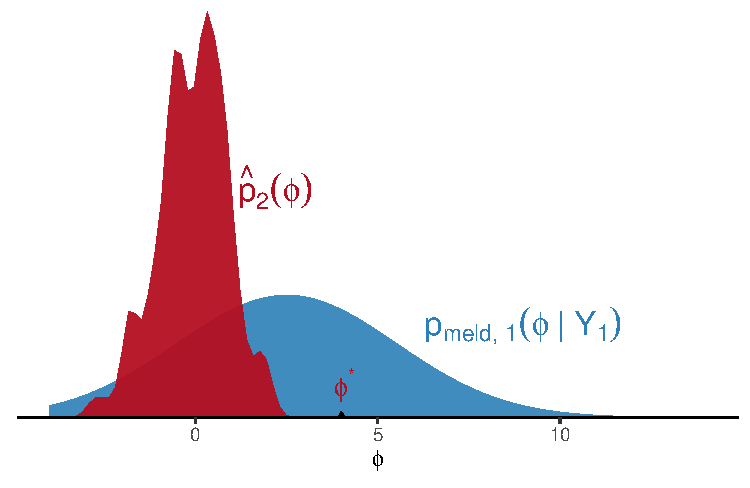
\includegraphics[width=0.85\linewidth]{figures/conflict} \end{center}

\end{frame}

\begin{frame}{Conflict in action}

\begin{equation*}
  \alpha (\phi^{*}, \phi) = 
  \frac {
    \pd_{\text{pool}} (\phi^{*})
    \pd_{2}(\phi^{*}, \psi_{2}, Y_{2})
  } {
    \pd_{\text{pool}} (\phi)
    \pd_{2}(\phi, \psi_{2}, Y_{2})
  }
  \cdot
  \textcolor{myredhighlight}{
    \frac {
      \hat{\pd}_{2}(\phi)
    } {
      \hat{\pd}_{2}(\phi^{*})
    }
  }
\end{equation*}

\begin{center}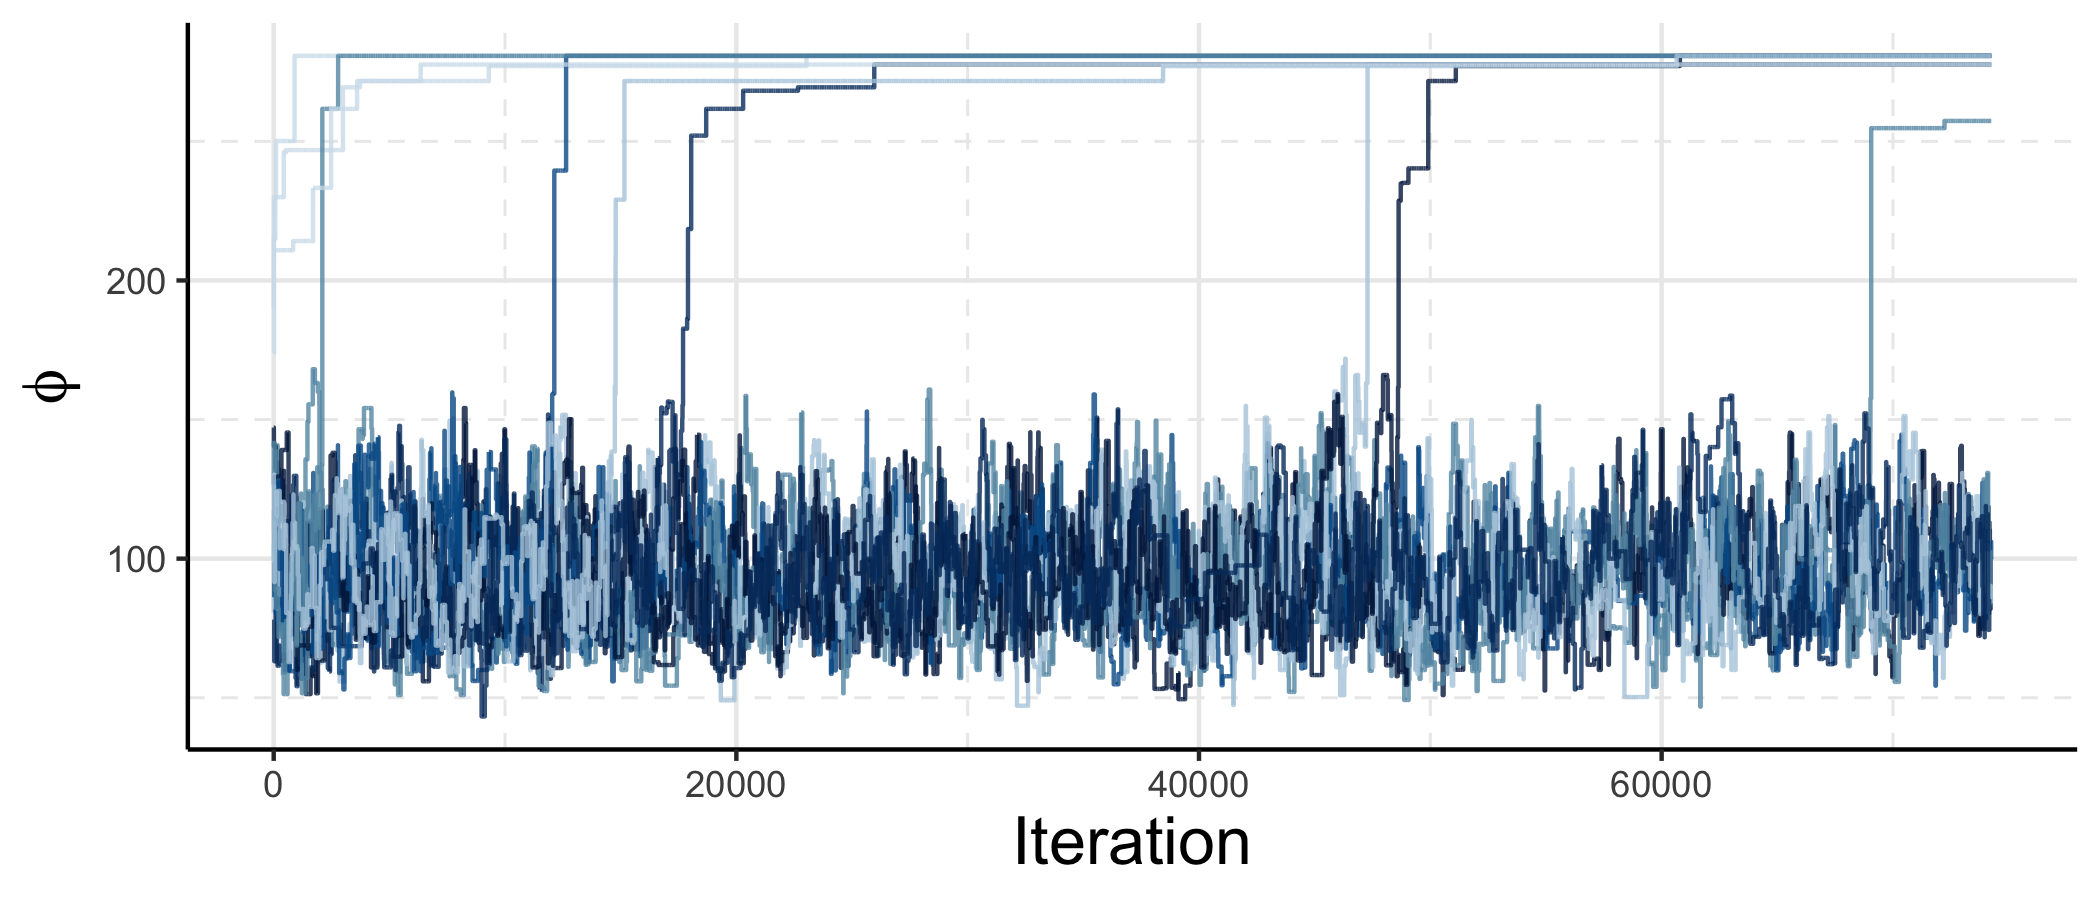
\includegraphics[width=1\linewidth]{figures/stage-two-trace-presentation-one} \end{center}

\begin{itemize}
\tightlist
\item
  H1N1 example from Goudie et al. (2019) 
\end{itemize}

\end{frame}

\begin{frame}{Self density ratios}

We only interact with unknown marginal via self-density ratio (Hiraoka,
Hamada, and Hori 2018):
\begin{equation*}
  \pdr(\phinu, \phide) = \frac {
    \pd(\phinu)
  } {
    \pd(\phide)
  }
  % \label{eqn:self-densit}
\end{equation*}

\emph{Weighted-sample self-density ratio estimation} (WSRE) Intuition:

\begin{itemize}
\tightlist
\item
  Sampling \(\phi \sim \pd(\phi, \psi, Y)\) admits
  \(\phi \sim \pd(\phi)\)
\item
  Instead, sample:\\
  \(\phi \sim \pd(\phi, \psi, Y) \w(\phi; \xi) \quad \rightarrow \quad \phi \sim \frac{1}{Z}\pd(\phi)\w(\phi; \xi) = \s(\phi)\)
\item
  Use the weighted sample density estimator of Jones (1991):
  \begin{equation*}
  {\textcolor{mymidblue}{\hat{\pd}}}(\phi) = 
  \frac{1}{\textcolor{mymidblue}{Z}Nh} 
    \sum\limits_{i=1}^{N} \w(\phi;\xi)^{-1} \text{K}_{h}(\phi - \phi_{i})
\end{equation*}
\item
  Ratio estimator is then:\\
  \begin{equation*}
  \pdrh(\phinu, \phide) = \frac{
    \textcolor{mymidblue}{\hat{\pd}}(\phinu)
  } {
    \textcolor{mymidblue}{\hat{\pd}}(\phide)
  }
\end{equation*}
\end{itemize}

\end{frame}

\begin{frame}{WSRE intuition - 1}

\begin{center}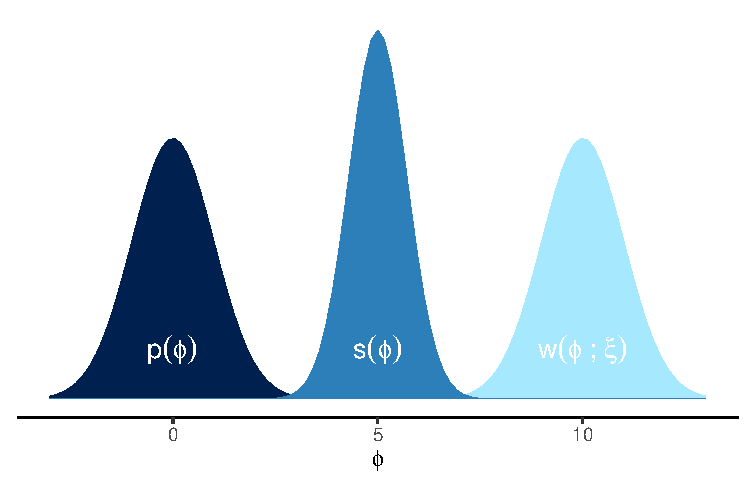
\includegraphics[width=1\linewidth]{figures/weighted-dist-plot} \end{center}

\end{frame}

\begin{frame}{WSRE intuition - \(\Nw\)}

\begin{center}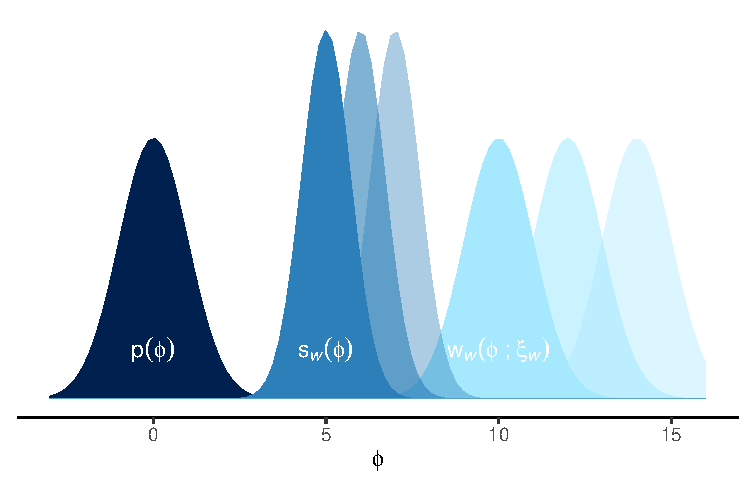
\includegraphics[width=1\linewidth]{figures/weighted-dist-plot-many} \end{center}

\end{frame}

\begin{frame}{H1N1 example - 2}

\begin{equation*}
  \alpha (\phi^{*}, \phi) = 
  \frac {
    \pd_{\text{pool}} (\phi^{*})
    \pd_{2}(\phi^{*}, \psi_{2}, Y_{2})
  } {
    \pd_{\text{pool}} (\phi)
    \pd_{2}(\phi, \psi_{2}, Y_{2})
  }
  \cdot
  \textcolor{mymidblue}{
    \pdrh(\phi, \phi^{*})
  }
\end{equation*}

\begin{center}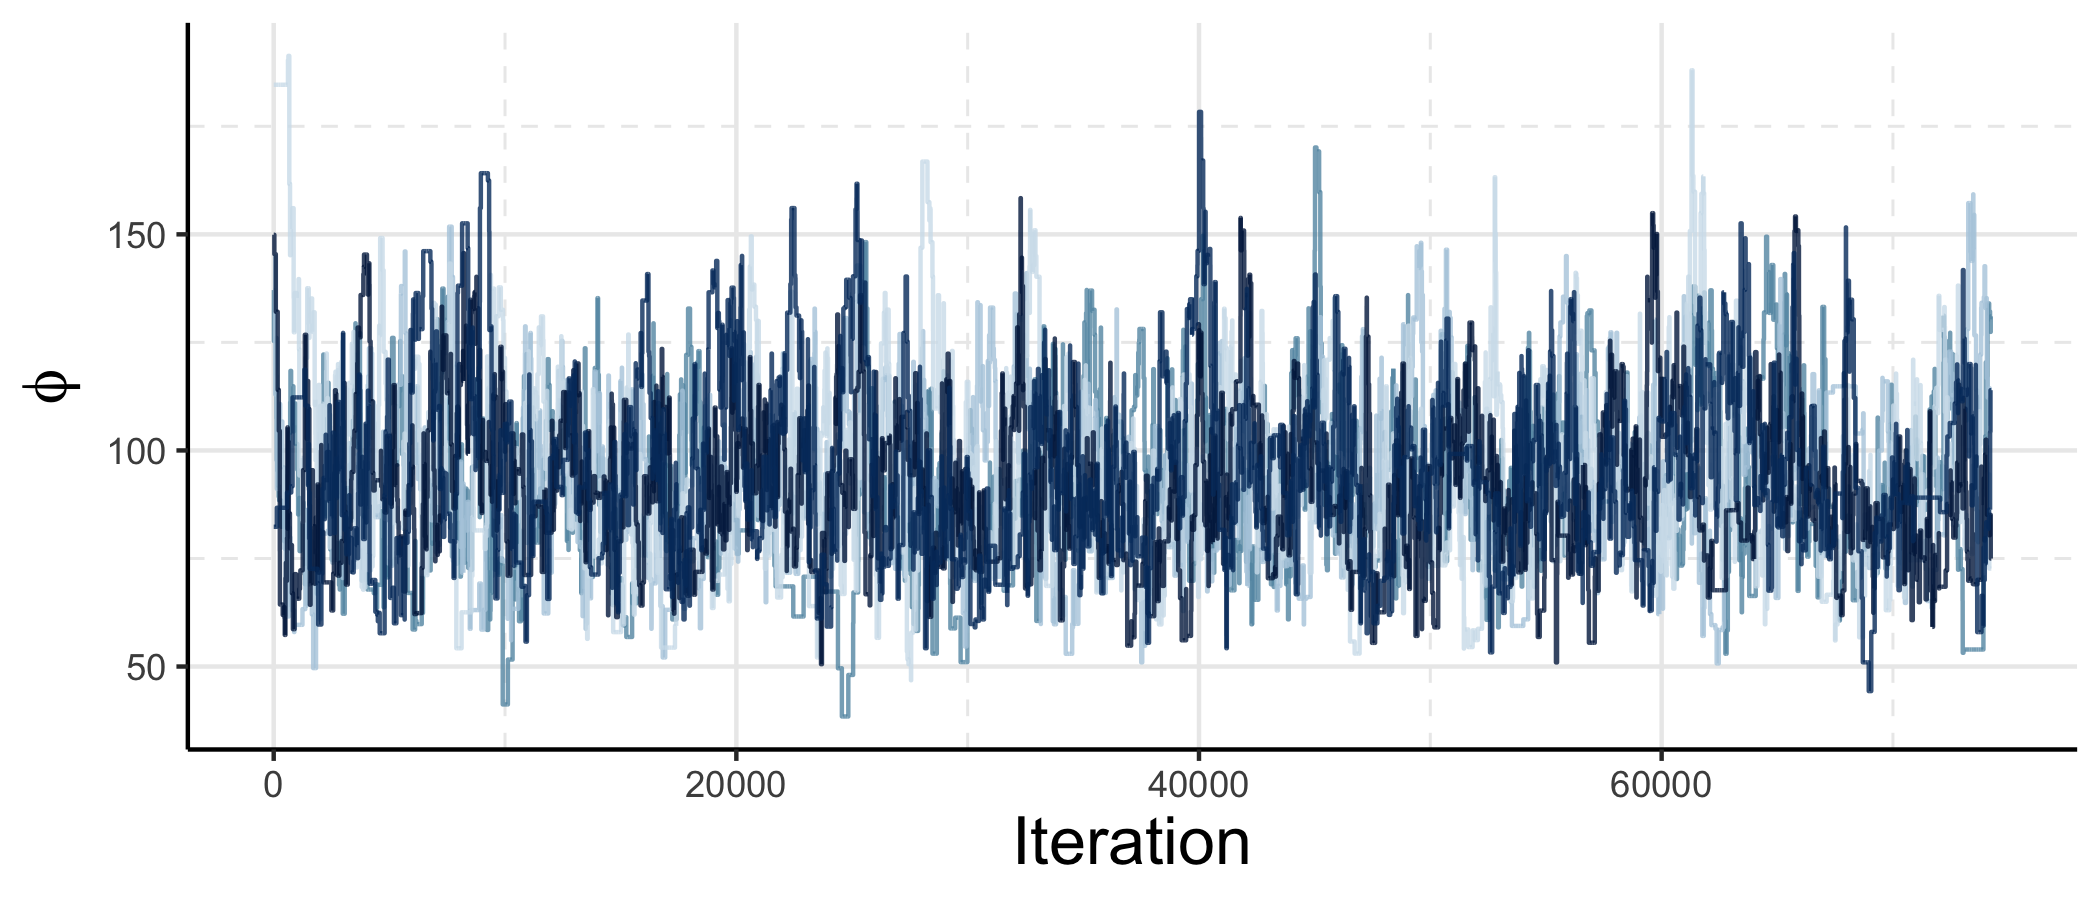
\includegraphics[width=1\linewidth]{figures/stage-two-trace-presentation-two} \end{center}

\end{frame}

\begin{frame}{Future plans}

\begin{itemize}
\tightlist
\item
  Markov melding for ICU delirium, using electronic health record data

  \begin{itemize}
  \tightlist
  \item
    Observational data (Temperature, respiratory rate)
  \item
    Blood test data
  \item
    Daily ICU drug dose data
  \item
    Each source is idiosyncratic \(\rightarrow\) requires substantial
    modelling effort (and domain expertise)
  \end{itemize}
\item
  Melding for multiple \(\phi\):
  \(\pd_{1}(\phi_{1}, Y_{1}) \,\,\,\, \pd_{2}(\phi_{1}, \phi_{2}, Y_{2}) \,\,\,\, \pd_{3}(\phi_{2}, Y_{3})\)
\item
  Addressing other kinds of internal difference in scale and location
  (conflict)
\end{itemize}

\end{frame}

\begin{frame}{Links}

Should you also wish to estimate self-density ratios:

\begin{itemize}
\tightlist
\item
  \url{https://github.com/hhau/wsre}
\end{itemize}

The traceplots are from this example:

\begin{itemize}
\tightlist
\item
  \url{https://github.com/hhau/full-melding-example}
\end{itemize}

This talk:

\begin{itemize}
\tightlist
\item
  \url{https://github.com/hhau/bsu-together-20mins}
\end{itemize}

\end{frame}

\begin{frame}{References}

\hypertarget{refs}{}
\hypertarget{ref-goudie:etal:18}{}
Goudie, Robert J. B., Anne M. Presanis, David Lunn, Daniela De Angelis,
and Lorenz Wernisch. 2019. ``Joining and Splitting Models with Markov
Melding.'' \emph{Bayesian Anal.} 14 (1). International Society for
Bayesian Analysis: 81--109.
doi:\href{https://doi.org/10.1214/18-BA1104}{10.1214/18-BA1104}.

\hypertarget{ref-hiraoka:hamada:hori:18}{}
Hiraoka, Kazuyuki, Toshihiko Hamada, and Gen Hori. 2018. ``Necessary and
Sufficient Conditions of Proper Estimators based on Self Density Ratio
for Unnormalized Statistical Models.'' \emph{Neural Networks} 98:
263--70.
doi:\href{https://doi.org/10.1016/j.neunet.2017.11.018}{10.1016/j.neunet.2017.11.018}.

\hypertarget{ref-jones:91}{}
Jones, M. C. 1991. ``Kernel Density Estimation for Length Biased Data.''
\emph{Biometrika} 78 (3). Oxford University Press, Biometrika Trust:
511--19. \url{http://www.jstor.org/stable/2337020}.

\end{frame}

\end{document}
